\chapter{Speech Emotion Recognition Using Acoustic Features}
% \section{Introduction}
The purpose of this chapter is two-fold: (1) to investigate the effective 
region of analysis for acoustic feature extraction, whether frame-based region
(local features) or utterance-based region (global features); and (2) to
evaluate the
effect of silence in dimensional speech emotion recognition. The latter issue
is taken by investigating the effectiveness of removing silence vs. using
silence as features. As auxiliary task, we performed an evaluation of
aggregating acoustic features at input stage and compared the result with the
baseline which is performed by aggregating output labels.

\section{SER using Low-level Acoustic Features}
% introduce frame-based processing
SER in conventional ways are performed by extracting acoustic features on
frame-based processing and then applied these features to a classifier. Let
$y(n)$, with $ n = 1, 2, 3, \ldots , L$, denotes acoustic signal with length
$L$.  In frame-based processing, this $y(n)$ signal is divided into frames by
fixed length. A typical length for a single frame is 16-25 milliseconds (ms)
with 10 ms to 15 ms hop length (stride). For 25 ms frame length and 10 ms hop
length, which is equal to 60\% overlap (15 ms), a window is applied to this
frame to make the short-time signal behave as quasistationary signal -- near
stationary signal. In their original length, an acoustic signal vary with the
time: non-stationary property.  Windowing processes acoustic signal in
short-term interval to remove this property. Figure \ref{fig:frame-processing}
shows the windowing process; short-term signals seems more stationary than the
original signal.

% # Windowing: why 25 ms, add figure, why overlapping

Windowing multiplies spectrum of input signal with window signal $w(n)$.  A
typical window function for acoustic signal is Hann and Hamming windows (named
after Julius von Hann and Richard W. Hamming).  The others are Rectangular,
Bartlet, Kaiser, and Blackman.  The choice of window function is based
on two aspects: width of main lobe and additional lobes. Hann and Hamming
windows only differ in weighting factors with similar concept: cosine-sum
windows. 

\begin{equation}
  w[n] = A + B \cos \biggl(\frac {2\pi n}{M}\biggl), ~~~~~n = -M/2, \ldots, M/2
\end{equation}

\noindent where $A$ is $0.5$ for Hann and $0.54$ for Hamming. $B$ is $0.5$ for
Hann and $0.46$ for Hamming. Both window functions are widely used in speech
processing due to good trade-off between time and frequency resolution (effect
of side lobes). Figure \ref{fig:window_hann} shows Hann window and its spectrum,
while Figure \ref{fig:windowing_demo} shows an example of Hamming window applied
to sinusoid signal and its result.

\begin{figure}[htbp]
  \centering
  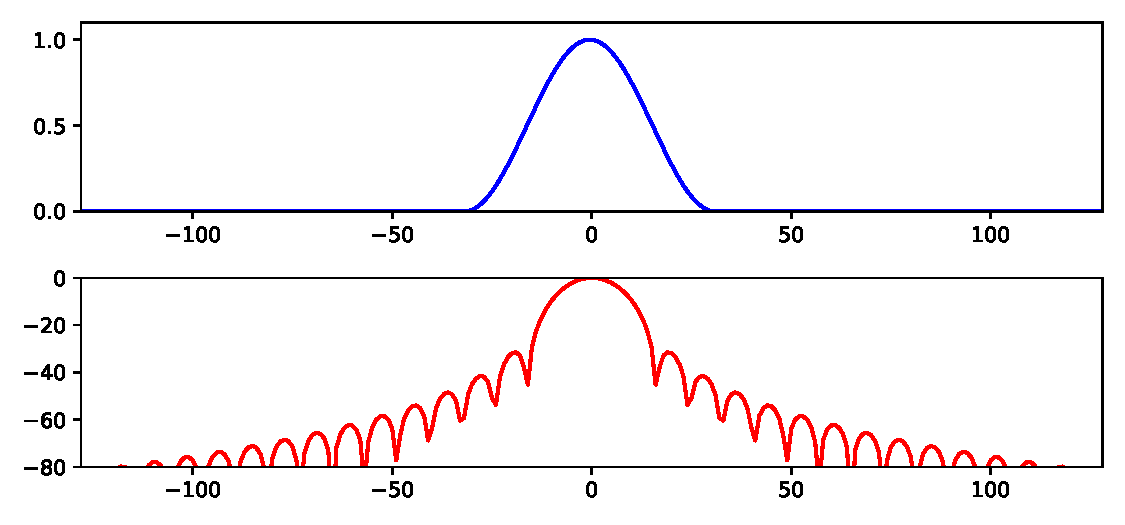
\includegraphics[width=\textwidth]{../fig/window_hann.pdf}
  \caption{Hann window and its spectrum}
  \label{fig:window_hann}
\end{figure}

\begin{figure}[htbp]
  \centering
  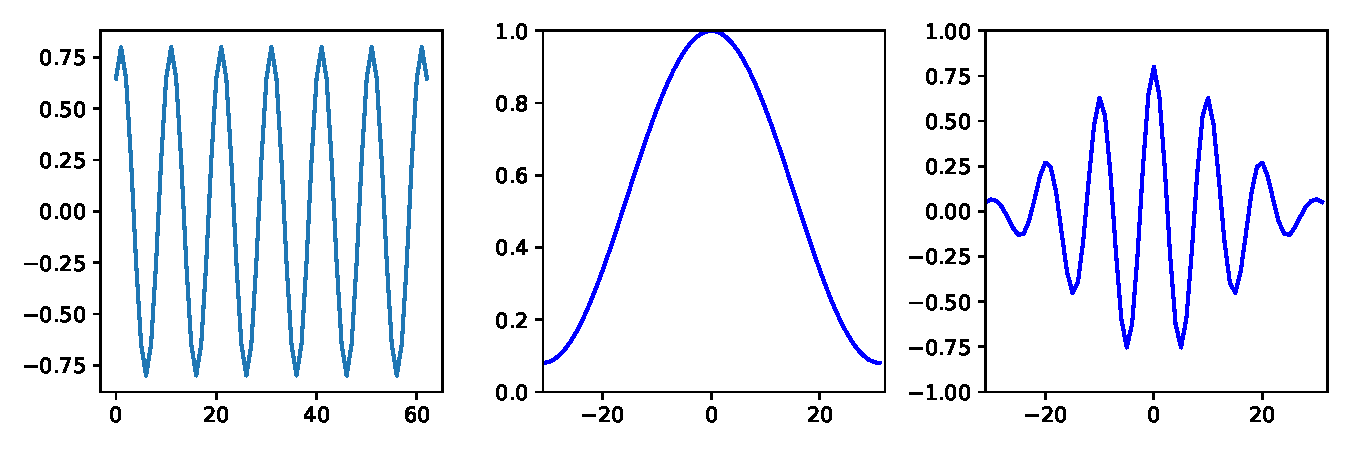
\includegraphics[width=\textwidth]{../fig/windowing_demo.pdf}
  \caption{An example of Hamming window (middle) applied to sinusoid signal (left); the resulted windowed signal (right) is multiplication of both.}
  \label{fig:windowing_demo}

\end{figure}
The length of a window is usually equal to the length of frame: one window per
frame. If the length of a window is smaller than a frame, each frame will be
windowed with window length and padded with zeros to match length of frame. It
costs more computation. In speech emotion recognition, short window is used to
capture short dynamics context while longer window is used to capture mid and
longer dynamics. A common approach used short window to extract acoustic
features in short-term time while long-term dynamics are modeled by statistical 
functions. Figure \ref{fig:frame-processing} shows frame-based processing of an
acoustic signal (speech) which windows short-term signals using Hamming window.

\begin{figure}[htbp]
  \centering
  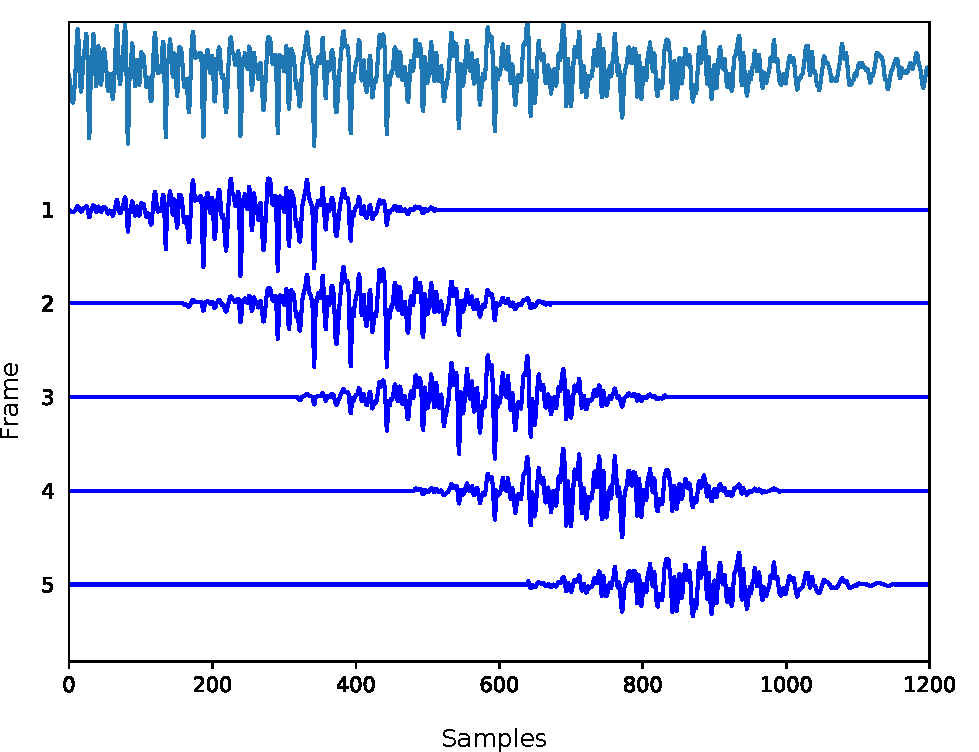
\includegraphics[width=\textwidth]{../fig/framing.pdf}  
  \caption{Frame-based processing for extracting low-level descriptors of an acoustic signal; the signal is an excerpt of IEMOCAP utterance with 400 samples frame length and 160 samples hop length; sampling frequency is 16 kHz.}
  \label{fig:frame-processing}
\end{figure}

% # LLD, MFCC, Why
The acoustic features extracted on each frame are known as local features or
low-level descriptor (LLD) \cite{Herrera1999}. The most common LLD for speech
processing is mel-frequency cepstral coefficients (MFCC). MFCC captures
different aspects of the spectral shape of a speech. The following steps
compute MFCC in sequences. First, FFT/DFT transformed time domain signal into
frequency domain signal (spectra). Second, mel frequency warping function
convert spectra in linear scale into mel scale. Although several functions have
been proposed, a common approach keeps linear scale for acoustic frequencies
below 1 kHz and converts to logarithmic scale for acoustic frequencies above 1
kHz. This conversion imitates human perceptual system. Third, convert a power
spectrogram (amplitude squared) to decibel (dB) units ($\log$). Finally, DCT
computes MFCC as amplitude cepstra.

% number of mfcc coefficients; number of frame; shape of MFCC
One of the important parameters in MFCC is the number of coefficients. A number
of 13 to 40 coefficients are common for speech processing. For
each frame 13 MFCCs are extracted. If there are 40 frames in an utterance, the
dimension of MFCC features will be (40, 13). Obviously, the number of frames
corresponds to the number of samples divided by hop length (in samples). 
If an utterance comprises 1 second (s) with 16000 Hz sampling rate, the
number of samples is 16000. Using 25 ms (400 samples) window/frame length and
10 ms (160 samples) hop length, the number of frames is $16000/160$, i.e.,
100 frames. Figure \ref{fig:mfcc_40} shows an MFCC spectrogram of an utterance
with 40 coefficients.

% mel-spectrogram and log mel-spectrogram
Recently, researchers found that mel-spectrogram, also called as (mel) filter
bank and mel frequency spectral coefficients (MFSC) for deep learning-based
automatic speech recognition (ASR) (e.g., \cite{Mohamed2014}). Given that deep
learning system is less susceptible with high correlated input, the DCT step in
previous MFCC calculation is not necessary since it is linear transformation.
DCT discards some information in speech signals which are highly non-linear
\cite{fayek2016}. Furthermore, a logarithmic version of mel-spectrogram, i.e.,
log mel-spectrogram, is preferable one since deep learning learns better in
this scale. The mel-spectrogram visualization as shown in Figure
\ref{fig:mfsc_128} support this argument in comparison with MFCC visualization.

% GeMAPS
Apart from the use of one type acoustic features for speech processing, some
researchers have proposed a set of acoustic features for speech emotion
recognition. Eyben et al. \cite{Eyben} proposed Geneva minimalistic parameter
set (GeMAPS) as standard acoustic features for affective voice research. The
proposed acoustic features are based on: (1) physiological changes in voice
production, (2) proven significance in previous studies, and (3) theoretical
significance. The proposed acoustic features comprises 23 LLDs as shown in
Table \ref{tab:gemaps_paa}. This acoustic feature set is extracted on
frame-processing basis with 25 ms frame length and 10 ms hop length.

% pyAudioanalysis
Giannakopulos \cite{Giannakopoulos2015} proposed pyAudioanalysis as an open
source Python library for audio signal analysis. The library supports a wide
range of audio analysis procedures such as feature extraction, classification,
supervised and unsupervised segmentation, and visualization. Different from
GeMAPS feature set, pyAudioanalysis targets a wide range of voice application
like audio event detection, speech emotion recognition, music segmentation, and
health application. The short-term feature set, which is extracted on
frame-processing basis, consists of 34 LLDs. These LLDs are shown in Table 
\ref{tab:gemaps_paa}.

\begin{table}[htpb]
  \centering
  \caption{Acoustic feature sets: GeMAPS \cite{Eyben} and pyAudioAnalysis \cite{Giannakopoulos2015}. The numbers in parentheses indicate the total numbers of features (LLDs).}
  \begin{tabular}{p{7.5cm} p{7cm}}
  \hline
  \hspace{2.5cm}GeMAPs (23) & \hspace{1.5cm}pyAudioAnalysis (34) \\
  \hline
intensity, alpha ratio, Hammarberg index, spectral slope 0-500 Hz, spectral
slope 500-1500 Hz, spectral flux, 4 MFCCs, F0, jitter, shimmer,
harmonics-to-noise ratio (HNR), harmonic difference H1-H2, harmonic difference
H1-A3, F1, F1 bandwidth, F1 amplitude, F2, F2 amplitude, F3, and F3 amplitude.
& zero crossing rate, energy, entropy of energy, spectral centroid, spectral
spread, spectral entropy, spectral flux, spectral roll-off, 13 MFCCs, 12 chroma
vectors, chroma deviation.\\
  \hline
  \end{tabular}
  \label{tab:gemaps_paa}
 \end{table}

% Result

% Summary LLD and Problem with frame-based processing: high-dimensions, needs
% zero padding

\section{SER using High-level Acoustic Features}

% \section{Evaluation Metric}
% \section{Experiment and Results on Region Analysis of Acoustic Features}
\section{Contribution of Silent Pause Features}
\section{Acoustic Features Aggregation}

% The content following two sections can be included in summary and previous
% sections
% \section{Effect of Different Acoustic Features}
% \section{Effect of Different Classifiers}
\section{Summary}

